%% ==========================================================================
%% Conference version (IEEEtran, target 6-8 pp).
%%
%% This is a genuine cut, not the journal paper with sections deleted: the
%% conference sections live in conf/ and are written tighter. It keeps ONE
%% lead contribution (extraction provenance) and the recovery trade, and
%% drops the fragility result, the congestion-model result, most of the
%% mechanism refutations, and most of the methods detail.
%%
%% If space is still short, cut in this order:
%%   1. Sec. "What adaptation contributes" (keep one sentence in Discussion)
%%   2. Table I (describe in prose)
%%   3. Fig. 2 (the provenance argument survives on Fig. 1 alone)
%% ==========================================================================
\documentclass[conference]{IEEEtran}

\usepackage[T1]{fontenc}
\usepackage[utf8]{inputenc}
\usepackage{graphicx}
\usepackage{amsmath}
\usepackage{amssymb}
\usepackage{booktabs}
\usepackage{url}

\graphicspath{{figures/}{../../figures/ieee/}}

\begin{document}

\title{What Does Self-Healing Routing Actually Buy?\\
Physarum and Ant Colony Optimization on a\\
Real Urban Road Network}

% House style matches the author's previous IEEE submission: name,
% department, institution, city/country, USN. Add further
% \IEEEauthorblockN/\IEEEauthorblockA pairs (separated by \and) for
% co-authors or a faculty mentor if required.
\author{%
\IEEEauthorblockN{N Litheesh}
\IEEEauthorblockA{Dept. of Computer Science and Engineering\\
RV College of Engineering\\
Bengaluru, India\\
1RV25CS107}%
}

\maketitle

\begin{abstract}
Bio-inspired routing methods are claimed to \emph{self-heal}: to adapt from
retained internal state after a disruption rather than recompute. That claim
is usually evaluated on synthetic undirected graphs without congestion, and
rarely by measuring recovery. We benchmark Dijkstra/A*, a MAX--MIN Ant
System, and a Physarum conductivity model on the real road network of
central Bengaluru (2{,}856 nodes, 7{,}015 directed edges, mean out-degree
2.46) under SUMO-simulated congestion, across seven closure scenarios and
warm- versus cold-start recovery: 5{,}520 runs, fully paired. We report two
results. First, \emph{path extraction decides what a Physarum number means}:
pooled, the model matches the optimum on 90\% of undisrupted pairs, but
using only its own maximum-flux walk the figure is 23.3\%, and on warm
recoveries it returns the Dijkstra fallback's path on 66.8\% of cells; the
median stretch is exactly 1.000 inside every provenance class, so a pooled
figure cannot be falsified. Second, \emph{warm start is a trade}: it cuts
recovery 2.97$\times$ in iterations and 6.87$\times$ in wall-clock
($n=358$, $p<10^{-51}$), with 48.3\% of warm recoveries converging in one
iteration where cold start never does, yet it is significantly worse on the
reported path ($p=4.3\times10^{-7}$). We argue the sparse directed structure
of a real road network is what exposes these effects, and that they are
structurally unreachable on the complete and near-complete undirected graphs
used in prior evaluations.
\end{abstract}

\begin{IEEEkeywords}
Bio-inspired routing, ant colony optimization, Physarum polycephalum,
network resilience, traffic simulation, benchmarking.
\end{IEEEkeywords}

\section{Introduction}

Ant colony optimization (ACO)~\cite{dorigo1996ant,stutzle2000maxmin} and
Physarum polycephalum conductivity
models~\cite{nakagaki2000maze,tero2007mathematical} maintain internal state
--- a pheromone field, a field of tube conductivities --- that is claimed to
let them adapt to a changed network rather than recompute from scratch. On a
road network, where closures and congestion change edge costs continuously,
that is an attractive property.

It is also rarely measured. Evaluations of these methods overwhelmingly use
synthetic graphs that are undirected and comparatively dense, report accuracy
on an undisrupted shortest-path problem, and treat the adaptive machinery as
self-evidently useful. Three gaps follow: the test graphs lack the structure
that makes real road routing hard (one-way streets, low out-degree,
cul-de-sacs); congestion is usually absent, so the weights the adaptation
tracks never move; and recovery after disruption --- the behaviour the
retained state exists to provide --- is seldom the measured quantity.

We close those gaps for one city. We benchmark Dijkstra and
A*~\cite{dijkstra1959note,hart1968formal}, a MAX--MIN Ant System, and a
Tero-style Physarum model on the real road network of central Bengaluru
under congestion from the SUMO microsimulator~\cite{lopez2018microscopic},
measuring recovery from seven classes of closure under warm start (retained
state) and cold start (state reset). Every algorithm sees identical OD
pairs, closures and traffic, and all quality figures use a Dijkstra optimum
computed on the same weighted graph.

\textbf{Contribution 1: extraction provenance, not the model, decides what a
Physarum result means.} The conductivity model emits a field, not a route; a
separate extraction step produces the path. Instrumenting that step shows
Physarum's apparent competence is largely its fallback's. Pooled, it matches
the optimum on 90.0\% of undisrupted pairs, reproducing the literature;
restricted to its own maximum-flux walk, 23.3\%. The median stretch is
exactly 1.000 in \emph{every} provenance class, so a pooled number cannot
distinguish the model from its Dijkstra fallback. On warm recoveries the
fallback supplies 66.8\% of reported paths.

\textbf{Contribution 2: warm start buys speed and charges quality.} It cuts
recovery 2.97$\times$ in iterations and 6.87$\times$ in wall-clock, paired
($n=358$); 48.3\% of warm recoveries converge in exactly one iteration,
which cold start never does. Per-iteration cost is unchanged, so the saving
is adaptation rather than cheaper arithmetic. Against this, warm start is
significantly worse on the reported post-disruption path
($p=4.3\times10^{-7}$) and completes its own extraction far less often.

We report what the methods lose as well as what they gain: Dijkstra
recomputes an exact route in one iteration and about 31\,ms, and no method
here approaches it on wall-clock.

\section{Related Work}

\textbf{Physarum shortest path.} The slime mould resolves a maze into the
shortest connecting path~\cite{nakagaki2000maze}; Tero et al.\ formalised
this as adapting conductivities driven by a Poiseuille-flow pressure
solve~\cite{tero2007mathematical}, later used to reproduce Tokyo rail-like
networks~\cite{tero2010rules}. Bonifaci et al.\ proved convergence to the
shortest path for \emph{undirected} graphs~\cite{bonifaci2012physarum}. The
directedness restriction is explicit in the literature: Zhang et al.\ note
the model is designed only for undirected networks and propose a directed
formulation~\cite{zhang2014directed}, which we do not implement. Our results
therefore characterise the canonical model on a directed network, an acknowledged
limitation, rather than reporting a defect.

\textbf{The prior three-way comparison.} Combining Physarum, ACO and
Dijkstra is not new. Zhang et al.\ benchmark exactly these
three~\cite{zhang2014improved}, reporting that their Physarum variant and
Dijkstra both attain optimal paths ``with one hundred percent'' while ACO
degrades with network size, on Erd\H{o}s--R\'enyi graphs of 15--2{,}000
nodes with static weights, no congestion and no disruption. Two points
matter. Their method needs \emph{no} extraction machinery, since the path is read
straight off the flux field, which separates cleanly on such graphs, so we
cannot claim that Physarum evaluations generally conflate provenance;
the honest contrast is that extraction is a formality there and decisive
here. And their ACO reaches zero optimal-path accuracy beyond 1{,}000 nodes,
whereas ours attains 43--44\% exact match on a larger and harder network,
which establishes our ACO as a strong baseline by the standard of the prior
art.

\textbf{Extraction and termination.} Wang et al.\ define a dominant-path
procedure procedurally identical to our maximum-flux
walk~\cite{wang2021transition}, and state that at convergence it yields
exactly the shortest path. On our network it yields a directed-legal path on
43.0\% of solves and the optimum on 23.3\%. The results are compatible: their
examples are complete graphs and small-worlds of mean degree 6--600, assumed
undirected, where the walk \emph{cannot} dead-end. Our network has mean
out-degree 2.46 with pervasive one-ways.

\textbf{ACO on traffic networks.} Zhang et al.\ propose orientation
guidance weighting edges by angular alignment with the
destination~\cite{zhang2018novel}, evaluated on one 528-node network with
static travel times against conventional ACO only; our goal-directed
ablation is related but distinct and we extend rather than contradict it.
Tuan et al.\ report an improved ACO beating conventional ACO, Dijkstra and a
genetic algorithm~\cite{tuan2026improved}, but evaluate on METR-LA under
fluctuating traffic~\cite{li2018diffusion} without measuring recovery after a
closure.

\textbf{Position.} A systematic pass over the open citation databases,
including complete forward-citation sweeps of
both~\cite{zhang2014improved} and~\cite{watanabe2011traffic}, returns no
study combining the three families on a real road network under
simulator-generated congestion with closure recovery as a measured outcome;
no work pairing Physarum with SUMO was found at all. The contribution
claimed here is the substrate and the measurement, not the three-algorithm
combination, which~\cite{zhang2014improved} already reported.

\section{Method}

\subsection{Network and congestion}

We study a $\sim$4$\times$4\,km area of central Bengaluru (MG Road, Cubbon
Park, Shivajinagar, Richmond Town), chosen for its irregular organically
grown topology. The network comes from OpenStreetMap via
OSMnx~\cite{boeing2017osmnx}, reduced to its largest strongly connected
component: \textbf{2{,}856 nodes, 7{,}015 directed edges, mean out-degree
2.46}. That last figure is the decisive structural property: a node with out-degree
two offers a walk-based extraction almost no choice, and one-way
streets mean a direction favoured by an undirected flow computation may be
illegal.

Algorithms never see the congestion source directly: a provider returns a
snapshot mapping each edge to a congested travel time. The primary source is
SUMO~\cite{lopez2018microscopic} at light and heavy synthetic demand, joined
to graph edges through OSM way IDs at \textbf{97.53\% coverage}. An analytic
BPR volume-delay function~\cite{bpr1964} is retained as an independent
secondary source.

Two details affect correctness. Because \texttt{netconvert} splits ways that
OSMnx merges, per-edge times must be aggregated in \emph{pace},
$t_e = \ell_e \sum_i t_i / \sum_i \ell_i$; averaging the matched segments'
travel times instead made 26\% of edges imply speeds above the network
maximum and silently broke A*'s admissibility. And free-flow speeds are
re-annotated from the generated SUMO network so numerator and denominator share one road model, which raises mean free-flow
speed to 51.5\,km/h, so
\textbf{absolute times here are optimistic and only ratios are reported}.

\subsection{Algorithms}

Dijkstra~\cite{dijkstra1959note} on the congested weight supplies the
reference cost for every stretch figure; A*~\cite{hart1968formal} uses a
great-circle/max-speed heuristic and is verified equal to Dijkstra rather
than assumed so.

\textbf{MMAS}~\cite{stutzle2000maxmin} uses $\tau^{\alpha}\eta^{\beta}$ with
$\eta = 1/t_{uv}$ and bounded pheromone. Plain MMAS does not work here: with
mean out-degree 2.46 the ant completion rate was \emph{zero}, so we
construct tours with backtracking plus a dead-node memo, raising completion
from 36\% to 80\%. The memo is lossy by measurement (about 66\% of prunes refuse a still-viable
node), and we document it as a deliberate heuristic.
A goal-directed variant using A*'s heuristic is reported as an ablation, not
the default: giving ACO target-location information Physarum never receives
would make the comparison unfair, and it is also not better.

\textbf{Physarum} carries conductivity $D_e$ and cost $L_e$ per edge, giving
conductance $w_e = D_e/L_e$. Each iteration solves a weighted-Laplacian
system for pressures (grounded at the sink), computes fluxes
$Q_e = w_e \Delta p_e$, and adapts
$D_e \leftarrow D_e + \mathrm{d}t\,(f(|Q_e|) - D_e)$ with
$f(Q)=|Q|^{\mu}/(1+|Q|^{\mu})$~\cite{tero2007mathematical}. Convergence is
$\max_e|\Delta D_e| < \epsilon$. \textbf{Pressures are solved on an
undirected projection while an extracted path must be directed-legal}, which
is the origin of most of what follows.

\textbf{Extraction, and its provenance.} The model yields a field, not a
route. We extract in three stages and record which produced the reported
path: (i) the \emph{maximum-flux walk}, stepping to the highest-flux
admissible successor with a visited set, the model's own extraction,
procedurally identical to~\cite{wang2021transition}; (ii) a shortest-path
search on the $D_e > \theta$ subgraph if the walk dead-ends; (iii) a
shortest-path search on the whole graph otherwise, which \emph{is plain Dijkstra}. Recording provenance per run is what makes
Section~\ref{sec:cprov} possible; without it a Physarum stretch of 1.000 is
unfalsifiable.

Under warm start we zero severed edges' conductivity, drop them from the
Laplacian and retain the rest; cold start resets $D$ to uniform. Closures
remove edges but not nodes, so a stranded node yields a singular Laplacian
and non-finite pressures, under which every flux and threshold comparison
silently fails and extraction falls through to the Dijkstra fallback. We
restrict the Laplacian to the source's connected component in the surviving
graph; we rejected an epsilon floor on $D$, which would invent transport
capacity across a closed road.

\subsection{Design and statistics}

Seven scenarios: no disruption (S0); one random path edge (S1); the
highest-betweenness path edge (S2); three (S3) and five (S4) simultaneous
path edges; a corridor, i.e. one named OSM way (S5); and an intersection
with all incident edges (S6). Closures are chosen relative to the current
optimal path, must leave the pair connected, and rejected candidates are
counted.

The matrix is 30 OD pairs (stratified by distance, disjoint from all tuning
draws) $\times$ 7 scenarios $\times$ 2 demand levels $\times$ \{warm,
cold\}: \textbf{5{,}520 runs}. ACO gets five seeds; Physarum one, justified
by measurement (three initialisation seeds gave costs identical to four
decimal places). All algorithms in a cell share one Dijkstra denominator.

Distributions are right-skewed and, for warm Physarum, bimodal, so we report
\textbf{median and IQR, never means}, with paired Wilcoxon signed-rank
tests~\cite{wilcoxon1945individual} on identical (OD, scenario, level, seed)
tuples and a two-stage clustered bootstrap (10{,}000 resamples) for
intervals. Pre-disruption quality is deduplicated on the initial solve,
which is identical across scenarios and start modes.

\section{Results}

The sweep completed 5{,}520 runs with 28 failures (0.51\%), all one cause:
two cells where no five path edges could be closed without disconnecting the
pair. All stretch invariants hold with zero violations.

\subsection{Extraction provenance decides what a Physarum number means}
\label{sec:cprov}

Pooled across extraction methods, Physarum matches the optimal route on
\textbf{90.0\%} of undisrupted pairs at heavy demand and 86.7\% at light,
reproducing the accuracy this model is credited with. Restricted to its own
maximum-flux walk, the same solves give \textbf{23.3\% and 16.7\%}. The walk
produces any path at all on 69.8\% of Physarum rows.

\begin{table}[t]
\caption{Provenance of Physarum's reported path (776 successful rows). The
median stretch is 1.000 in \emph{every} class.}
\label{tab:cprov}
\centering
\begin{tabular}{lrrrr}
\toprule
Extraction method & Own? & $n$ & Share & Exact \\
\midrule
\texttt{full\_graph\_fallback}     & no  & 315 & 40.6\% & 95.2\% \\
\texttt{max\_flux\_walk}           & yes & 232 & 29.9\% & 74.6\% \\
\texttt{theta\_subgraph\_fallback} & no  & 229 & 29.5\% & 94.3\% \\
\bottomrule
\end{tabular}
\end{table}

About \textbf{70\% of reported Physarum paths did not come from its own
extraction}, and \texttt{full\_graph\_fallback} is plain Dijkstra. Since the
median stretch is exactly 1.000 within each class
(Table~\ref{tab:cprov}), a pooled median cannot separate ``the model found
the optimum'' from ``the fallback returned Dijkstra's answer'', and a pooled
Physarum-versus-Dijkstra comparison is partly circular.

On recovery the effect is sharper and \emph{mode-dependent}. Cold start
splits walk/threshold/full-graph as 95/201/62 (17.3\% Dijkstra); warm start
as 119/\textbf{0}/\textbf{239}. With roughly 98.8\% of retained tubes below
$\theta$, warm's threshold subgraph never connects the pair, a hard zero across all
358 cells, so \textbf{warm Physarum reports plain Dijkstra's
path on two-thirds of recoveries}.

Fig.~\ref{fig:cconv} is the clearest evidence: in two of three panels the
with-fallback curve sits at stretch 1.0 from iteration one, because it was
Dijkstra's answer before the model did any work. We therefore report
Physarum as two labelled series throughout and never pool them.

\begin{figure*}[t]
\centering
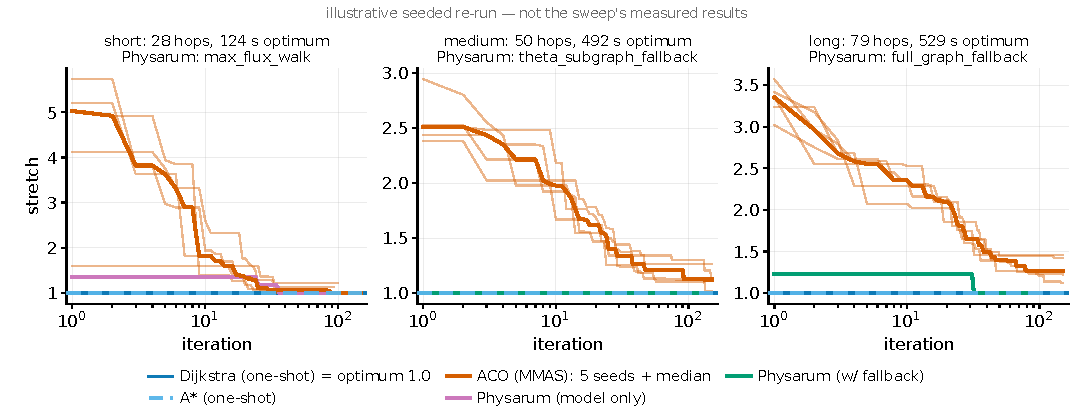
\includegraphics[width=\figw]{fig01_convergence.pdf}
\caption{Cost versus iteration across three distance strata. The Physarum
with-fallback series starts at stretch 1.0 in two of three panels: that is
the fallback, not convergence.}
\label{fig:cconv}
\end{figure*}

For context, ACO reaches 43.3\%/44.0\% exact match with median stretch
1.0052 (light) and 1.0209 (heavy), and Dijkstra and A* are exact by
construction. ACO \emph{misses} the exit criterion we set in advance
(stretch $\leq 1.10$ on $\geq 90\%$ of pairs), reaching 73.3\% under free
flow with a 95\% CI of [58.7, 86.7] entirely below the bar; the failure mode
is a colony settling on a wrong corridor, with MMAS's own convergence
criterion firing on most such solves. We report this rather than retuning
until it passes.

\subsection{Warm start buys speed and charges quality}

\begin{table}[t]
\caption{Recovery cost, scenarios S1--S6. Dijkstra is the honest baseline:
no method here approaches it on wall-clock.}
\label{tab:crecovery}
\centering
\small
\begin{tabular}{llrrrr}
\toprule
Algorithm & Start & $n$ & Iters & Wall (s) & 1 iter \\
\midrule
Dijkstra  & cold & 358 & 1.0 & 0.031 & 100\% \\
A*        & cold & 358 & 1.0 & 0.027 & 100\% \\
ACO       & warm & 1790 & 69.0 & 34.07 & 0\% \\
ACO       & cold & 1790 & 110.0 & 59.80 & 0\% \\
Physarum  & warm & 358 & 42.0 & 0.235 & \textbf{48.3\%} \\
Physarum  & cold & 358 & 98.0 & 5.661 & 0\% \\
\bottomrule
\end{tabular}
\end{table}

Table~\ref{tab:crecovery} gives the raw cost, and the first thing it shows is
that \textbf{Dijkstra wins on wall-clock, which we report rather than hide}: a
recompute on this graph costs about 31\,ms where the bio-inspired methods take
seconds. The defensible quantities are iterations-to-adapt and
post-disruption quality.

Paired on identical cells, warm start cuts Physarum's recovery by
\textbf{2.97$\times$ in iterations} (faster on 350/358,
$p=3.2\times10^{-59}$) and \textbf{6.87$\times$ in wall-clock} (336/358,
$p=9.0\times10^{-52}$); ACO gains 1.26$\times$ and 1.56$\times$
($n=1{,}790$).

Two points matter more than the ratios. The distribution is \textbf{bimodal,
not merely shifted}: 48.3\% of warm recoveries converge in exactly one
iteration while cold start never does and its minimum is 73
(Fig.~\ref{fig:cwc}). The ratio of the two medians is therefore not a valid statistic; an earlier version of this analysis computed one and produced
a spurious 24$\times$. And \textbf{per-iteration cost is essentially
identical} warm versus cold (0.0511 vs 0.0538\,s), establishing that the
saving is fewer iterations rather than cheaper ones.

\begin{figure*}[t]
\centering
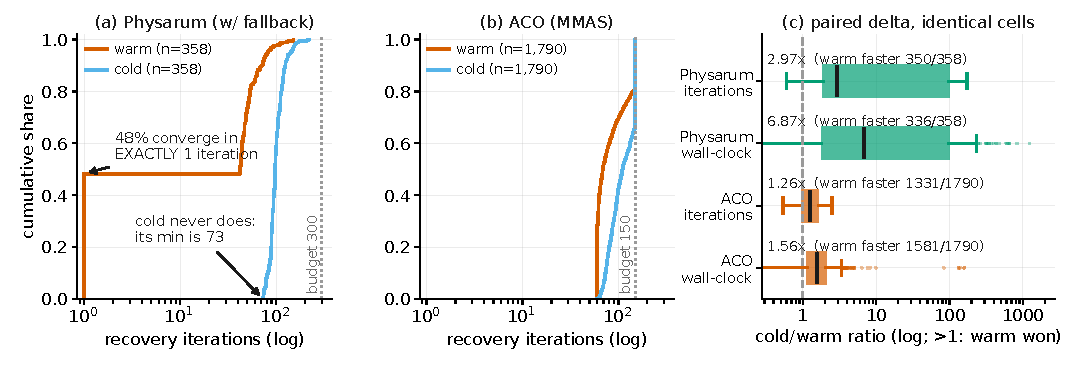
\includegraphics[width=\figw]{fig07_warm_vs_cold.pdf}
\caption{Warm versus cold recovery. The mode at exactly one iteration is the
shape of the result and the reason we report paired ratios.}
\label{fig:cwc}
\end{figure*}

\textbf{The cost.} On the reported path, paired across all 358 cells, cold
start is better: cold wins 57, warm 11, 290 ties
($p=4.3\times10^{-7}$). On the model's own extraction, the warm walk
completes on only 36.3\% of recoveries against cold's 59.5\%. Reporting the
speed-up alone describes half the effect.

\textbf{Why.} We tested the obvious mechanism, a retained field driving flux down severed
corridors, and \emph{refuted} it: a placebo closure at
least eight hops away reproduces nearly the whole deficit and is
indistinguishable from a closure directly on the route (43.3\% vs 41.7\%,
$n=60$ paired, $p=1.00$). A second candidate, that warm start leaves less
conductivity, is \emph{analytically impossible}: scaling $D$ by $c$ scales
$w$ by $c$ and $p$ by $1/c$, leaving $Q=w\Delta p$ unchanged (verified
numerically to $<10^{-15}$). What the data support is that \textbf{the walk
works on a near-uniform field and stops working as the field converges onto
a thin corridor}: convergence alone, with no closure, drops completion from
69.8\% to 43.0\%, and cold start's advantage is that it rewinds the field to
a walkable state.

\begin{figure*}[t]
\centering
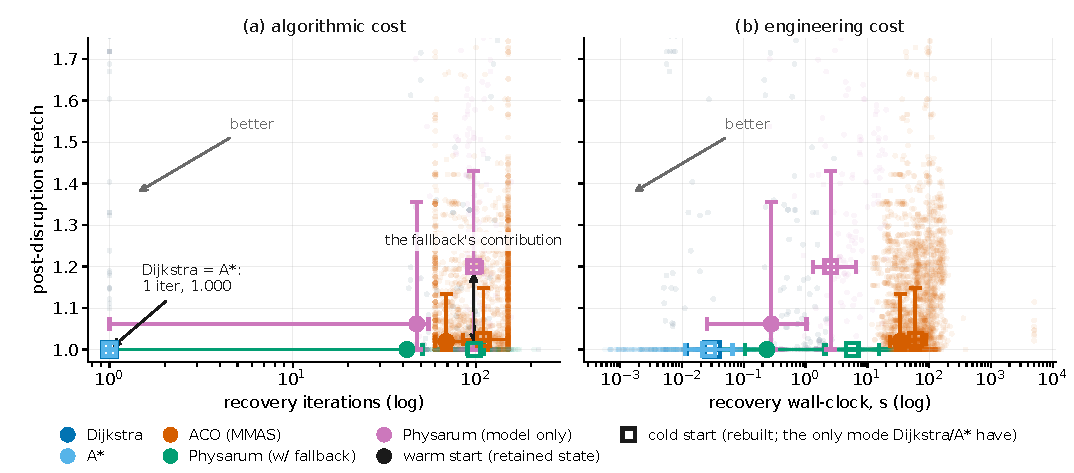
\includegraphics[width=\figw]{fig04_pareto_recovery_vs_quality.pdf}
\caption{The speed-versus-quality trade. Markers are medians with IQR arms
over the individual S1--S6 recovery runs; Dijkstra and A* anchor the lower
left. The model-only and pooled Physarum series share the same runs, so
\emph{the vertical gap between them is the fallback's contribution}.}
\label{fig:cpareto}
\end{figure*}

\subsection{What adaptation contributes}

This invites the conclusion that the model should stop earlier. Against a zero-adaptation control (the same pressure solve on a uniform
field, containing none of the Tero dynamics, and exact by construction since
the solver extracts before updating $D$), the converged field completes
\emph{less} often (0.433 vs 0.567) yet is far better when it does (median
stretch \textbf{1.0059} vs 1.4367; exact given completion 46.2\% vs 5.9\%).
Paired, the unadapted field loses 26--0 to the best adapted iteration
($n=34$, $p=8.3\times10^{-6}$), reproducing at scale on cold recovery
(120--1, $p=3.2\times10^{-21}$).

\textbf{Completion and quality move in opposite directions}, because a
near-uniform field is walkable precisely \emph{because} it is uninformative.
This also resolves the tension with~\cite{wang2021transition}: their claim
concerns quality, which does improve with convergence; what fails here is
completion, which a complete graph cannot exhibit. Consequently \textbf{no
earlier stopping rule is worth adopting}: a perfect per-cell oracle buys
\emph{zero} additional exact matches, since every exact-match walk is
already exact at convergence, and the router already retains the best walk
across iterations.

\subsection{The congestion model decides the sign of the effect}

On the undisrupted solve, ACO's within-10\% rate is 81.3\% under light SUMO
demand and 58.0\% under heavy, and paired on the same (OD, seed) cells heavy
is significantly worse ($p=0.036$; 37 pairs pass only under light against 2
only under heavy).

This \emph{reverses} what we measure on the analytic BPR provider, where
congestion improves ACO's outcomes because it flattens the cost surface so
more routes land within 10\% of optimal. The algorithm, the network and the
OD pairs are identical; only the congestion source differs. SUMO puts signal
delay in the numerator but not the free-flow denominator, while BPR loads
synthetic demand onto shortest paths, which is exactly where an OD-path
measurement walks.

\textbf{So the sign of the congestion effect is a property of the congestion
model, not of the algorithm}, and any claim about routing behaviour ``under
congestion'' that does not name its congestion model is underdetermined. We
accordingly retract a framing from our own earlier analysis, that the two
bio-inspired methods fail in opposite directions under congestion, which held
on BPR and does not survive SUMO, where both degrade.

\section{Discussion}

\textbf{Why a real road network was necessary.} The maximum-flux walk fails
by \emph{dead-ending}: reaching a node with no admissible unvisited
successor. On a complete graph that is impossible, and on a small-world of
mean degree 6--600 it is vanishingly rare. Our network has mean out-degree
2.46, and the undirected pressure solve routinely prefers a direction the
road forbids, so the failure mode we measure is structurally unreachable on
the substrates where this model's accuracy was established. That reframes
the disagreement with prior work as a matter of domain rather than
correctness: neither \cite{zhang2014improved} nor \cite{wang2021transition}
is wrong on its own graphs. What changes on a directed, sparse, organically
grown network is that extraction stops being a formality and becomes the
step that decides the reported outcome.

\textbf{Provenance as a reporting requirement.} A Physarum accuracy figure
on such a network is a statement about the extraction policy at least as
much as about the model, and a pooled number is unfalsifiable, since our
90\% and our 23.3\% come from the same solves. Any evaluation of this model
class on a directed network should publish the provenance distribution of
its reported paths, and a model whose fallback is a shortest-path algorithm
should report what share of its results that fallback produced. The stakes
are concrete: the stranded-component degeneracy of Section~\ref{sec:method}
produced a fabricated mean stretch of exactly 1.000 on the scenario where
the model is weakest, with no error raised, and provenance instrumentation
is what made it visible.

\textbf{What self-healing is worth here.} The adaptive state is real and
substantial: single-iteration recovery on nearly half of all closures, at
unchanged per-iteration cost, which is the strongest form of the claim we
can support. But it is paid for in path quality, on both the reported path
and the model's own extraction. A system that must guarantee route quality
after a closure should prefer a cold solve or a recompute; one that must
respond within a single adaptation step and can tolerate a few percent of
path cost is where retained state pays. Neither conclusion follows from the
speed measurement alone. And the baseline stands: Dijkstra recomputes an
exact route in about 31\,ms here, so at this network size recomputation is
simply the right engineering answer, and the case for adaptive methods must
rest on regimes we did not test: far larger networks, many simultaneous
commodities, or settings where the cost function is not globally observable.

\textbf{Limitations.} One city and one bounding box, so the structural
properties we argue are decisive, while common to dense organically grown
cities, are not demonstrated to transfer. Congestion comes from synthetic
demand rather than calibrated counts, which is where the closest recent ACO
work is stronger~\cite{tuan2026improved}; we traded measured demand for a
controlled, repeatable closure protocol over a full directed street network.
Absolute times are optimistic because the shared baseline re-annotates
free-flow speeds, so we report only ratios. Physarum is run per OD pair
rather than as multi-commodity flow, and we did not implement the directed
formulation~\cite{zhang2014directed}, so our findings characterise the
canonical model on a directed network, an acknowledged limitation of that
model, rather than the limits of Physarum-style methods in principle. ACO
was tuned while Physarum was near-default, a real asymmetry, though the
extraction findings concern a structural failure mode rather than a
parameter setting.

\section{Conclusion}

Benchmarking classical, ant-colony and Physarum routing on a real directed
road network under microsimulated congestion, over 5{,}520 paired runs, we
find that the self-healing claim holds in its strongest form, and that it is
a trade: warm start recovers in a single iteration on 48.3\% of closures,
which cold start never achieves and at unchanged per-iteration cost, yet is
significantly worse on the reported post-disruption path. The finding we
think matters most is methodological. A Physarum model emits a field, not a
route, and on a sparse directed network the extraction step decides the
answer: pooled, our Physarum matches the optimum on 90\% of pairs; using
only its own walk, 23.3\%. Because the median stretch is exactly 1.000
inside every provenance class, a pooled figure cannot be falsified, so we
argue provenance should be reported as a matter of course. Throughout,
Dijkstra remained the honest baseline that no method here approached on
wall-clock.


\bibliographystyle{IEEEtran}
\bibliography{refs}

\end{document}
